\section{Análisis Organizacional}
%MARITO

\subsection{Estructura Organizacional}
%MARITO

La estructura organizacional que utilizará \emph{Music Labs}
será la horizontal, pues debido al tamaño de la empresa no tiene 
sentido realizar una gran verticalidad en los cargos. Además, en este 
tipo de empresas, se requiere respuestas rápidas, y buen contacto
de la ``plana mayor'' con todos los trabajadores, lo cual se complica 
teniendo una estructura vertical, debido a la burocracia que puede 
existir al momento de tomar una decisión importante. Esta estructura básicamente
consiste en mantener un administrador de tiempo completo, junto a su secretario(a), 
que será quien tiene a cargo la empresa. Sobre él recaerá cada una de las unidades 
de la organización, que se dedican a un área específica. 
\begin{figure}[h!t]
   \centering
  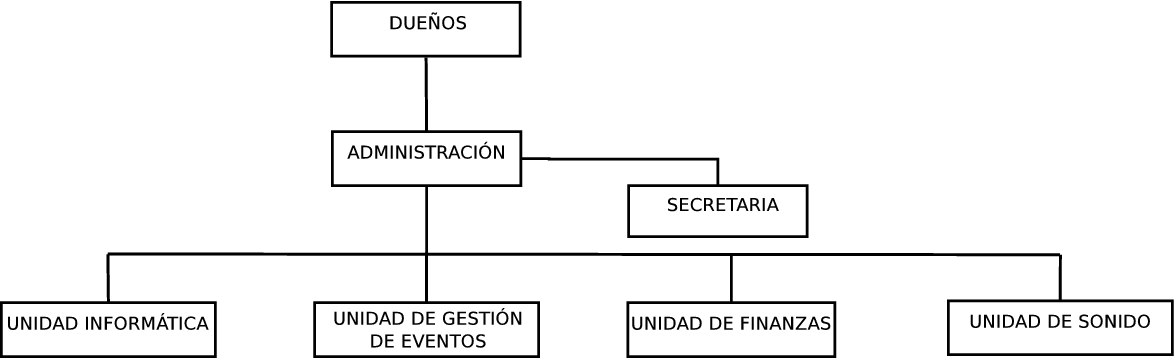
\includegraphics[scale=0.4]{img/estructuraorganizacional.png}
   \caption{Estructura organizacional}
   \label{fig:Estructura organizacional}
\end{figure}

A continuación se detallan cada una de las áreas de la estructura
organizacional:

\begin{itemize}

	\item Dueños: Corresponden a las personas dueñas del negocio en sí. Pueden (o no)
	permanecer en el lugar en que la organización se desempeña. Son los dueños del capital
	inicial, y a quienes deben rendirle cuentas cada una de las unidades de la empresa.

	\item Administrador: De preferencia, este cargo debe recaer en un
	 Ingeniero Industrial, Comercial, de Proyectos, o similar. Su función principal
	consiste en la coordinación de las 4 unidades que se encuentran bajo su cargo. Además, debe 
	velar por el buen funcionamiento de la empresa, y entregar reportes relevantes a los dueños, 
	en caso de ser requeridos. 
	
	\item Secretario(a): Entregar el apoyo que sea necesario al administrador. Además, todas 
	las solicitudes de sala de ensayo, estudio de grabación, entre otras, serán gestionadas por él.

	\item Encargado Unidad Informática: De preferencia, este cargo debe recaer en un 
	Ingeniero Informático o similar. Su función principal es la de encargarse de los clientes
	que solicitan el apoyo de posicionamiento en la web 2.0. En caso de verse sobrepasado por 
	las bandas que requieren de este servicio, está facultado para contratar (en base a 
	honorarios) a programadores que puedan realizar el trabajo, previo aviso al administrador.

	\item Encargado Unidad de Finanzas: De preferencia, este cargo debe recaer en un Ingeniero
	Comercial, o en un Contador. Su función principal consiste en estar al tanto de todos los 
	movimientos financieros que se realicen dentro de la empresa, además de la declaración de 
	los impuestos en el momento en que corresponda. Otra tarea a cumplir, es la de estar
	a cargo de las remuneraciones de las personas que trabajan dentro de \emph{Music Labs}.

	\item Encargado Unidad de Gestión de Eventos: Su función principal es la de canalizar 
	las solicitudes de eventos por parte de las bandas. Estos eventos pueden ser realizados 
	tanto en locales externos, como de \emph{Music Labs}. Esto lleva a definir ciertas subtareas, 
	que son determinar el monto a pagar, cantidad de personas, equipos necesarios, etc.

	\item Encargado Unidad de Sonido: De preferencia, este cargo debe recaer en un Ingeniero 
	en Sonido, o similar. Su función principal es la de encargarse del funcionamiento de la
	sala de ensayo y el estudio de grabación. En particular, debe estar capacitado para poder
	asistir a las bandas al momento que decidan grabar sus discos. 

\end{itemize}

Cabe destacar que cada una de las unidades tiene personas a su cargo, pero estas personas son llamadas
según sea la necesidad de la empresa. No son funcionarios de planta. 

\subsection{Leyes laborales atingentes al proyecto}
%Javier

Para dejar claramente establecido, y en palabras del artículo 3 del Código del Trabajo\footnote{Código del
trabajo del Ministerio de Trabajo y Previsión Social}, se entiende por:

\begin{itemize}
  \item \textbf{Empleador}: la persona natural o jurídica que utiliza los servicios intelectuales o materiales
de una o más personas en virtud de un contrato de trabajo.
  \item \textbf{Trabajador}: toda persona natural que preste servicios personales intelectuales o materiales, bajo
dependencia o subordinación, y en virtud de un contrato de trabajo, y
  \item \textbf{Trabajador Independiente}: aquel que en el ejercicio de la actividad de que se trate no depende de 
empleador alguno ni tiene trabajadores bajo su dependencia.
\end{itemize}

En cuanto al contrato de trabajo la empresa se guiará por lo que dice el artículo 7: \emph{``Contrato individual de trabajo 
es una convención por la cual el empleador y el trabajador se obligan recíprocamente, éste a prestar servicios personales 
bajo dependencia y subordinación del primero, y aquél a pagar por estos servicios una remuneración determinada''}. El 
contrato debe tener, por lo menos, las siguientes estipulaciones:

\begin{enumerate}
  \item lugar y fecha del contrato;
  \item individualización de las partes con indicación de la nacionalidad y fechas de nacimiento e ingreso del trabajador;
  \item determinación de la naturaleza de los servicios y del lugar o ciudad en que hayan de prestarse;
  \item monto, forma y período de pago de la remuneración acordada;
  \item duración y distribución de la jornada de trabajo, salvo que en la empresa existiere el sistema de trabajo por turno, caso en el cual se estará a lo dispuesto en el reglamento interno;
  \item plazo del contrato, y
  \item demás pactos que acordaren las partes.
\end{enumerate}

Respecto al término de contrato de un trabajador estará normado por lo indicado en el artículo
159 del código del trabajo el cual dice que el trabajo terminará en los siguientes casos:

\begin{itemize}
  \item Mutuo acuerdo de las partes.
  \item Renuncia del trabajador, dando aviso a su empleador con treinta días de anticipación, a lo menos.
  \item Muerte del trabajador.
  \item Vencimiento del plazo convenido en el contrato. La duración del contrato de plazo fijo no podrá exceder de un año.
  \item Conclusión del trabajo o servicio que dio origen al contrato.
  \item Caso fortuito o fuerza mayor.
\end{itemize}

Además tal como indica el artículo 161: \emph{``Sin perjuicio de lo señalado en los artículos precedentes, 
el empleador podrá poner término al contrato de trabajo invocando como causal las necesidades de la empresa, 
establecimiento o servicio, tales como las derivadas de la racionalización o modernización de los mismos, bajas 
en la productividad, cambios en las condiciones del mercado o de la economía, que hagan necesaria la separación 
de uno o más trabajadores, y la falta de adecuación laboral o técnica del trabajador''}.\\

En razón de brindar un mejor servicio a los clientes, los trabajadores de la empresa tendrán capacitación
ocupacional acorde al trabajo realizado, siendo una capacitación ocupacional \emph{``el proceso destinado a promover, 
facilitar, fomentar y desarrollar las aptitudes, habilidades o grados de conocimientos de los trabajadores, con el 
fin de permitirles mejores oportunidades y condiciones de vida y de trabajo''}, tal como detalla el artículo 179.
Este tipo de capacitación será entregada en los términos que definen los artículos 180 al 183 del código del
trabajo.\\

Tal como lo estipula el artículo 13 del Código, solamente se contratarán personas mayores de edad, es decir,
personas con 18 años cumplidos o más.\\

Más detalles relacionados con la jornada de trabajo, remuneraciones, seguridad laboral y otros temas laborales están 
detallados en la sección 4 de este informe.

\subsection{Análisis de remuneraciones y sus proyecciones}

A continuación se detallan las remuneraciones que estarán disponibles en cada uno de los cargos
que se describieron anteriormente. Además, se detallará las remuneraciones a honorarios que pueden percibir
las personas que sean contratadas vía necesidad de la empresa.

Cabe destacar que los montos acá nombrados corresponden a la situación en que una persona distinta
esté a cargo de cada unidad nombrada, pero esto eventualmente puede cambiar, pues una misma persona 
perfectamente podría estar a cargo de la Unidad de Eventos y la Unidad de Sonido. En este caso, el sueldo 
final no correspondería a la suma de los 2 cargos, sino que al sueldo de uno de ellos multiplicado por 1.5

\begin{table}[h]
\centering
\begin{tabular}{|c|c|c|c|c|c|c|} \hline
Cargo           & Imponible & AFP      & Salud   & Accidentes & Cesantía & Líquido  \\ \hline
Administrador   & \$1200000 & \$148800 & \$84000 & \$11520    & \$28800  & \$926880 \\ \hline
Unidad Info     & \$1000000 & \$124000 & \$70000 & \$9600     & \$24000  & \$772400 \\ \hline
Unidad Finanzas & \$1000000 & \$124000 & \$70000 & \$9600     & \$24000  & \$772400 \\ \hline
Unidad Eventos  & \$1000000 & \$124000 & \$70000 & \$9600     & \$24000  & \$772400 \\ \hline
Unidas Sonido   & \$1000000 & \$124000 & \$70000 & \$9600     & \$24000  & \$772400 \\ \hline
Secretario(a)   & \$500000  & \$62000  & \$35000 & \$4800     & \$12000  & \$386200 \\ \hline
\end{tabular}
\caption{Sueldos del personal de planta}
\end{table}
En caso de necesitar profesionales o técnicos debido a una gran demanda de funciones (técnicos 
en sonido, programadores, comunicadores audiovisuales, etc), éstos serán trabajadores a honorarios, 
y su paga a recibir corresponderá a \$6000 bruto por hora trabajada, no debiendo exceder las 5 horas diarias de trabajo.

Cada uno de estos sueldos se reajusta de forma anual, en base a los indicadores nacionales más un 2\% sobre el sueldo del año.
Además, los dueños están en su derecho de entregar bonos de desempeño semestrales, en caso de ser necesario.

Si se realiza una proyección a los primeros 5 años en base sólo a sueldos de personal de planta, y sin contar el IPC
nacional, los montos que desembolsará la empresa serán los siguientes:

\begin{table}[h]
\centering
\begin{tabular}{|c|c|c|c|c|c|} \hline
              & Año 1     & Año 2     & Año 3     & Año 4     & Año 5     \\ \hline
Total a pagar & \$5700000 & \$5814000 & \$5930280 & \$6048886 & \$6169863 \\ \hline
\end{tabular}
\caption{Proyección de los sueldos totales a 5 años}
\end{table} 

Estos montos no incluyen al personal que será contratado por necesidad de la empresa, en caso
de que la demanda por parte de las bandas sea mucha. Además, cabe destacar que estos montos corresponden 
al costo Mensual durante el Año X.
\subsection{Tabla resumen de egresos (clasificándolos en inversiones y operacionales)}

La tabla de resumen de egresos corresponde a montos utilizados a lo más dentro del primer año. 
Estos egresos no necesariamente serán replicados en los años posteriores, pues las primeras inversiones
(material musical, instrumentos) no se renuevan año a año.

Para especificar cada uno de los egresos de \emph{Music Labs} se clasificará cada uno de ellos, antes de
mostrar la tabla correspondiente. 

\begin{enumerate}
	\item Costos operacionales
	\begin{enumerate}
		\item Costos Directos: Sueldos.
		\item Costos Indirectos: Si bien no se ha definido aún, el aseo externo puede ser un costo indirecto para la empresa
		\item Costos Fijos: Arriendo.
		\item Costos Variables: Gastos básicos (luz, agua, gas, teléfono)
		\item Gastos Generales: Insumos de oficina.
	\end{enumerate}

	\item Costos de inversión
	\begin{enumerate}
		\item Capital Fijo: Equipos de oficina, sala de ensayo, grabación, sala de eventos, adaptaciones.
		\item Capital Intangible: Costos de formación de sociedad (3.2\% del capital, ver punto 6.3). Suponiendo un capital 
		inicial de 100000000 (cien millones), correspondería a 3200000 (tres millones doscientos mil).
		\item Capital de Trabajo: El capital de trabajo se puede obtener mediante distintos métodos. Se mostrará inicialmente el método de desfase.

		$$
		\frac{\text{número de desfase}*\text{egresos 1º año}}{12}
		$$

		Como se puede apreciar, se toman en cuenta los egresos del primer año, que consideran los sueldos y remuneraciones, entre otras cosas. 
Como esta tabla en general se trata de egresos del primer año, y además, se detallan los costos operacionales por separado, no se considerará el capital de 
trabajo como un ítem separado.
\end{enumerate}
\end{enumerate}
% Arriendo                    & 12000  & 12000  & 12000  & 12000  & 12000  & 12000  & 12000  & 12000  & 12000  & 12000 \\
% Equipos de Oficina          & 655    & 0      & 0      & 0      & 0      & 0      & 367    & 150    & 0      & 0\\
% Equipos Sala de Ensayo      & 6045   & 0      & 0      & 0      & 0      & 0      & 6045   & 0      & 0      & 0 \\
% Equipos Grabación           & 3524   & 0      & 0      & 0      & 0      & 0      & 3524   & 0      & 0      & 0 \\
% Equipos Sala de eventos     & 6000   & 0      & 0      & 0      & 0      & 0      & 6000   & 0      & 0      & 0 \\
% Adaptaciones especializadas & 2616   & 0      & 0      & 0      & 0      & 0      & 0      & 0      & 0      & 0 \\
% Adaptaciones necesarias     & 8719   & 0      & 0      & 0      & 0      & 0      & 0      & 0      & 0      & 0  \\
% Materias primas e insumos   & 92718  & 92718  & 92718  & 92718  & 92718  & 92718  & 92718  & 92718  & 92718  & 92718 \\
% Total anual                 & 132277 & 104718 & 104718 & 104718 & 104718 & 104718 & 120649 & 104868 & 104718 & 104718 \\

%\red{cmaureir:} Estos son los elementos de la tabla de egresos del informe pasado,
%pero no veo como cosas de sueldos y esas cosas, que serían \emph{Costos Directos}
%además hay otros elementos de esta tabla que no tenemos ningún \emph{egreso},
%como lo son:
%\begin{itemize}
%   \item Capital Intangible
%   \item Capital de trabajo
%   \item Costos Indirectos
%   \item Gastos Generales
%   \item Costos Variables
%\end{itemize}
%
%Acá la categorización de los egresos que habíamos puesto en informe 2:
%
%\begin{itemize}
%   \item Arriendo (Costo fijo)                  
%   \item Equipos de Oficina (Capital Fijo)      
%   \item Equipos Sala de Ensayo (Capital Fijo)          
%   \item Equipos Grabación       (Capital Fijo)         
%   \item Equipos Sala de eventos (Capital Fijo)         
%   \item Adaptaciones especializadas (Capital Fijo)      
%   \item Adaptaciones necesarias    (Capital Fijo)      
%   \item Materias primas e insumos (Costos directos) 
%\end{itemize}
%
%\red{cmaureir:} fin comentario (comentado en el .tex están los tipos de elementos de cada punto)

\begin{table}[htb!]
\centering
%\small
\scriptsize
	\begin{tabular}{|l|r|r|}
      \hline
      {\bf Resumen de costos}      & Costo Mensual  & Costo Anual    \\ \hline
      \blue{Costos de Inversión}   &                &                \\ \hline
      Capital Fijo                 & 2297           & 27759          \\ \hline
      Capital Intangible           & -              & -              \\ \hline
      Capital de trabajo           & -              & 3200              \\ \hline
                                   & {\bf Total }   & {\bf 30959 }   \\ \hline
      \blue{Costos Operacionales}  &                &                \\ \hline
      Costos Directos              & 5700           & 68400          \\ \hline
      Costos Indirectos            & No considerado & No considerado \\ \hline
      Gastos generales             & 50             & 600            \\ \hline
      Costos Variables             & 932            & 11182          \\ \hline
      Costos fijos                 & 1000           & 12000          \\ \hline
                                   & {\bf Total }   & {\bf 92182 }   \\ \hline
   \end{tabular}
\caption{Resumen de egresos (en miles)}
\end{table}


%  Capital Fijo:
%     referido al costo de realización física del proyecto y está asociada a inversiones en:
%        -Compra de terrenos
%        -Adquisición de equipos
%        -Construcción de obras civiles
%        -Construcción de proyectos complementatios (alcantarillado, agua potable, tendido eléctrico, líneas telefónicas, etc)
%        -Cañerias, instrumentos, aislamiento.
%  
%  Capital en Intangible:
%     -Costos de ingeniería (asesoramiento técnico y supervisión)
%     -Gastos de administración
%     -Gastos de puesta en marcha
%     -Patentes y licencias
%     -Sistemas de información pre-operativos
%     -Seguros y costo de montaje
%     -Capacitación
%     -Estudios técnicos durante la ejecución
%  
%  Capital de Trabajo
%     Constituye el conjunto de recursos necesarios, en la
%     forma de activos circulantes, para la operación normal del proyecto
%     durante un ciclo productivo, para un tamaño determinado.
%    
%     Métodos de Estimación:
%        -El método contable
%        -El método del periodo de desfase
%        -El método del déficit acumulado máximo
%  
%  Costos Directos:
%     Materias primas y materiales directos
%     Mano de obra directa (incluye supervisión de operación hasta jefe de turno).
%     Comprende sueldos y salarios, gastos previsionales, horas extraordinarias,
%        bonos, incentivos y beneficios adicionales.
%     Insumos directos (energía, combustibles, lubricantes, vapor, agua,
%        refrigeración, etc., cuando corresponda)
%  
%  Costos Indirectos:
%     Mano de obra indirecta (supervisión y mantención general, seguridad
%        industrial, vigilancia, control de calidad, laboratorios, etc.)
%     Materiales Indirectos
%     Otros gastos indirectos (servicio médico, casino, movilización,
%        comunicaciones, iluminación, transporte interno, aseo de planta, etc.)
%     Beneficios del personal (jardín infantil, club de campo, economato, etc.)
%  
%  Gastos Generales:
%     Gastos administrativos (sueldos de personal ejecutivo, comunicaciones e
%        impresiones, aseo de oficinas, útiles de oficina, etc.)
%     Cargos fijos (seguros)
%     Gastos de ventas (sueldos, comisiones, gastos de representación, viáticos,
%        publicidad).
%     Investigación y desarrollo
%     Gastos de financiamiento (intereses y amortización del préstamo)
%  
%  Costos fijos:
%     son independientes del volumen de producción. Ej:
%     depreciación, arriendo, los costos de administración
%  
%  Costos variables:
%     dependen del volumen de producción, pues varían con
%     la producción. Ej: costos de energía eléctrica, de materias primas, ciertas
%     categorías de mano de obra, etc
%  
